\chapter{Methodisches Vorgehen}\label{chap:6}\largerpage[2]
Hinsichtlich des Umfangs des zu analysierenden Datenmaterials und der Dichte des Ortsnetzes musste zunächst die grundsätzliche Entscheidung zwischen einer quantitativ umfangreichen und einer qualitativ tiefgehenden Untersuchung getroffen werden. Ich habe mich für einen Kompromiss zwischen diesen beiden legitimen Forschungsinteressen entschieden, der eine in meinen Augen aussagekräftige, und zugleich machbare Lösung darstellt. Untersucht wurde das nominale Flexionssystem von 37 Tiefenbohrungspunkten in den oobd. Dialekten Bayerns. Ziel und Anspruch dieses Vorgehens ist es, durch ein Ortsnetz von Tiefenbohrungspunkten, die Nominalflexion in der arealen Dimension darzustellen und zugleich die Flexionssysteme der einzelnen Ortspunkte zu erfassen. Pro Ortspunkt war durch das umfangreiche Fragebuch des \textit{Bayerischen Sprachatlas} (und hierin speziell die Fragen zur Nominalflexion) eine qualitative Auswertung des Datenmaterials möglich. Durch die Dichte des BSA-Ortsnetzes können außerdem die Daten benachbarter Ortspunkte zum Vergleich herangezogen und die Analysen der einzelnen Tiefenbohrungspunkte durch weitere Datenpunkte abgesichert werden. Ergänzt wurde die primäre Materialbasis durch weitere Datenquellen (siehe \sectref{sec:6.2}), sodass für die einzelnen Tiefenbohrungspunkte (wo möglich) eine Kurzeitdiachronie aufgestellt werden konnte. \sectref{sec:6.1} gibt zunächst einen Überblick über die Auswahlkriterien des Untersuchungsgebiets (UG) und der einzelnen Tiefenbohrungspunkte. In \sectref{sec:6.3} wird schließlich die Methodik der Datenaufbereitung und -auswertung dargestellt.

\section{Untersuchungsgebiet und Tiefenbohrungspunkte}
\label{sec:6.1}
Gegenstand der Untersuchung sind die Darstellung und der Vergleich von Flexionssystemen einzelner Ortsdialekte des oobd. Dialektraumes. Wieso ist eine Fokussierung der oobd. Dialekte Bayerns sinnvoll? Zum einen ist dies durch die gute Datensituation für eine dialektvergleichende Untersuchung der Flexionsmorphologie in diesem Gebiet bedingt, zum anderen ergibt sich dies aus der Außenabgrenzung und der inneren Struktur des Dialektraums. So zeigt \citet{Lameli2013} mit einer raumstatistischen Reanalyse von Wredes Dialekteinteilungskarte, dass der oobd. Dialektraum in seiner Außenabgrenzung einen spezifischen, in sich geschlossenen Dialektraum bildet. Die drei Teilräume Ofr., Nord- und Mittelbair. wiederum weisen hinsichtlich ihrer phonologischen Strukturen sowohl Spezifika als auch Gemeinsamkeiten auf, was eine Untersuchung der Numerusflexion eines größeren Dialektraumes unter verschiedenen phonologischen Bedingungen in ihren Ähnlichkeiten und Unterschieden (ganz im Sinne eines Dialektlabors, siehe \chapref{chap:2}) ermöglicht (vgl. \citealt[3]{Rowley1997}).


\begin{map}
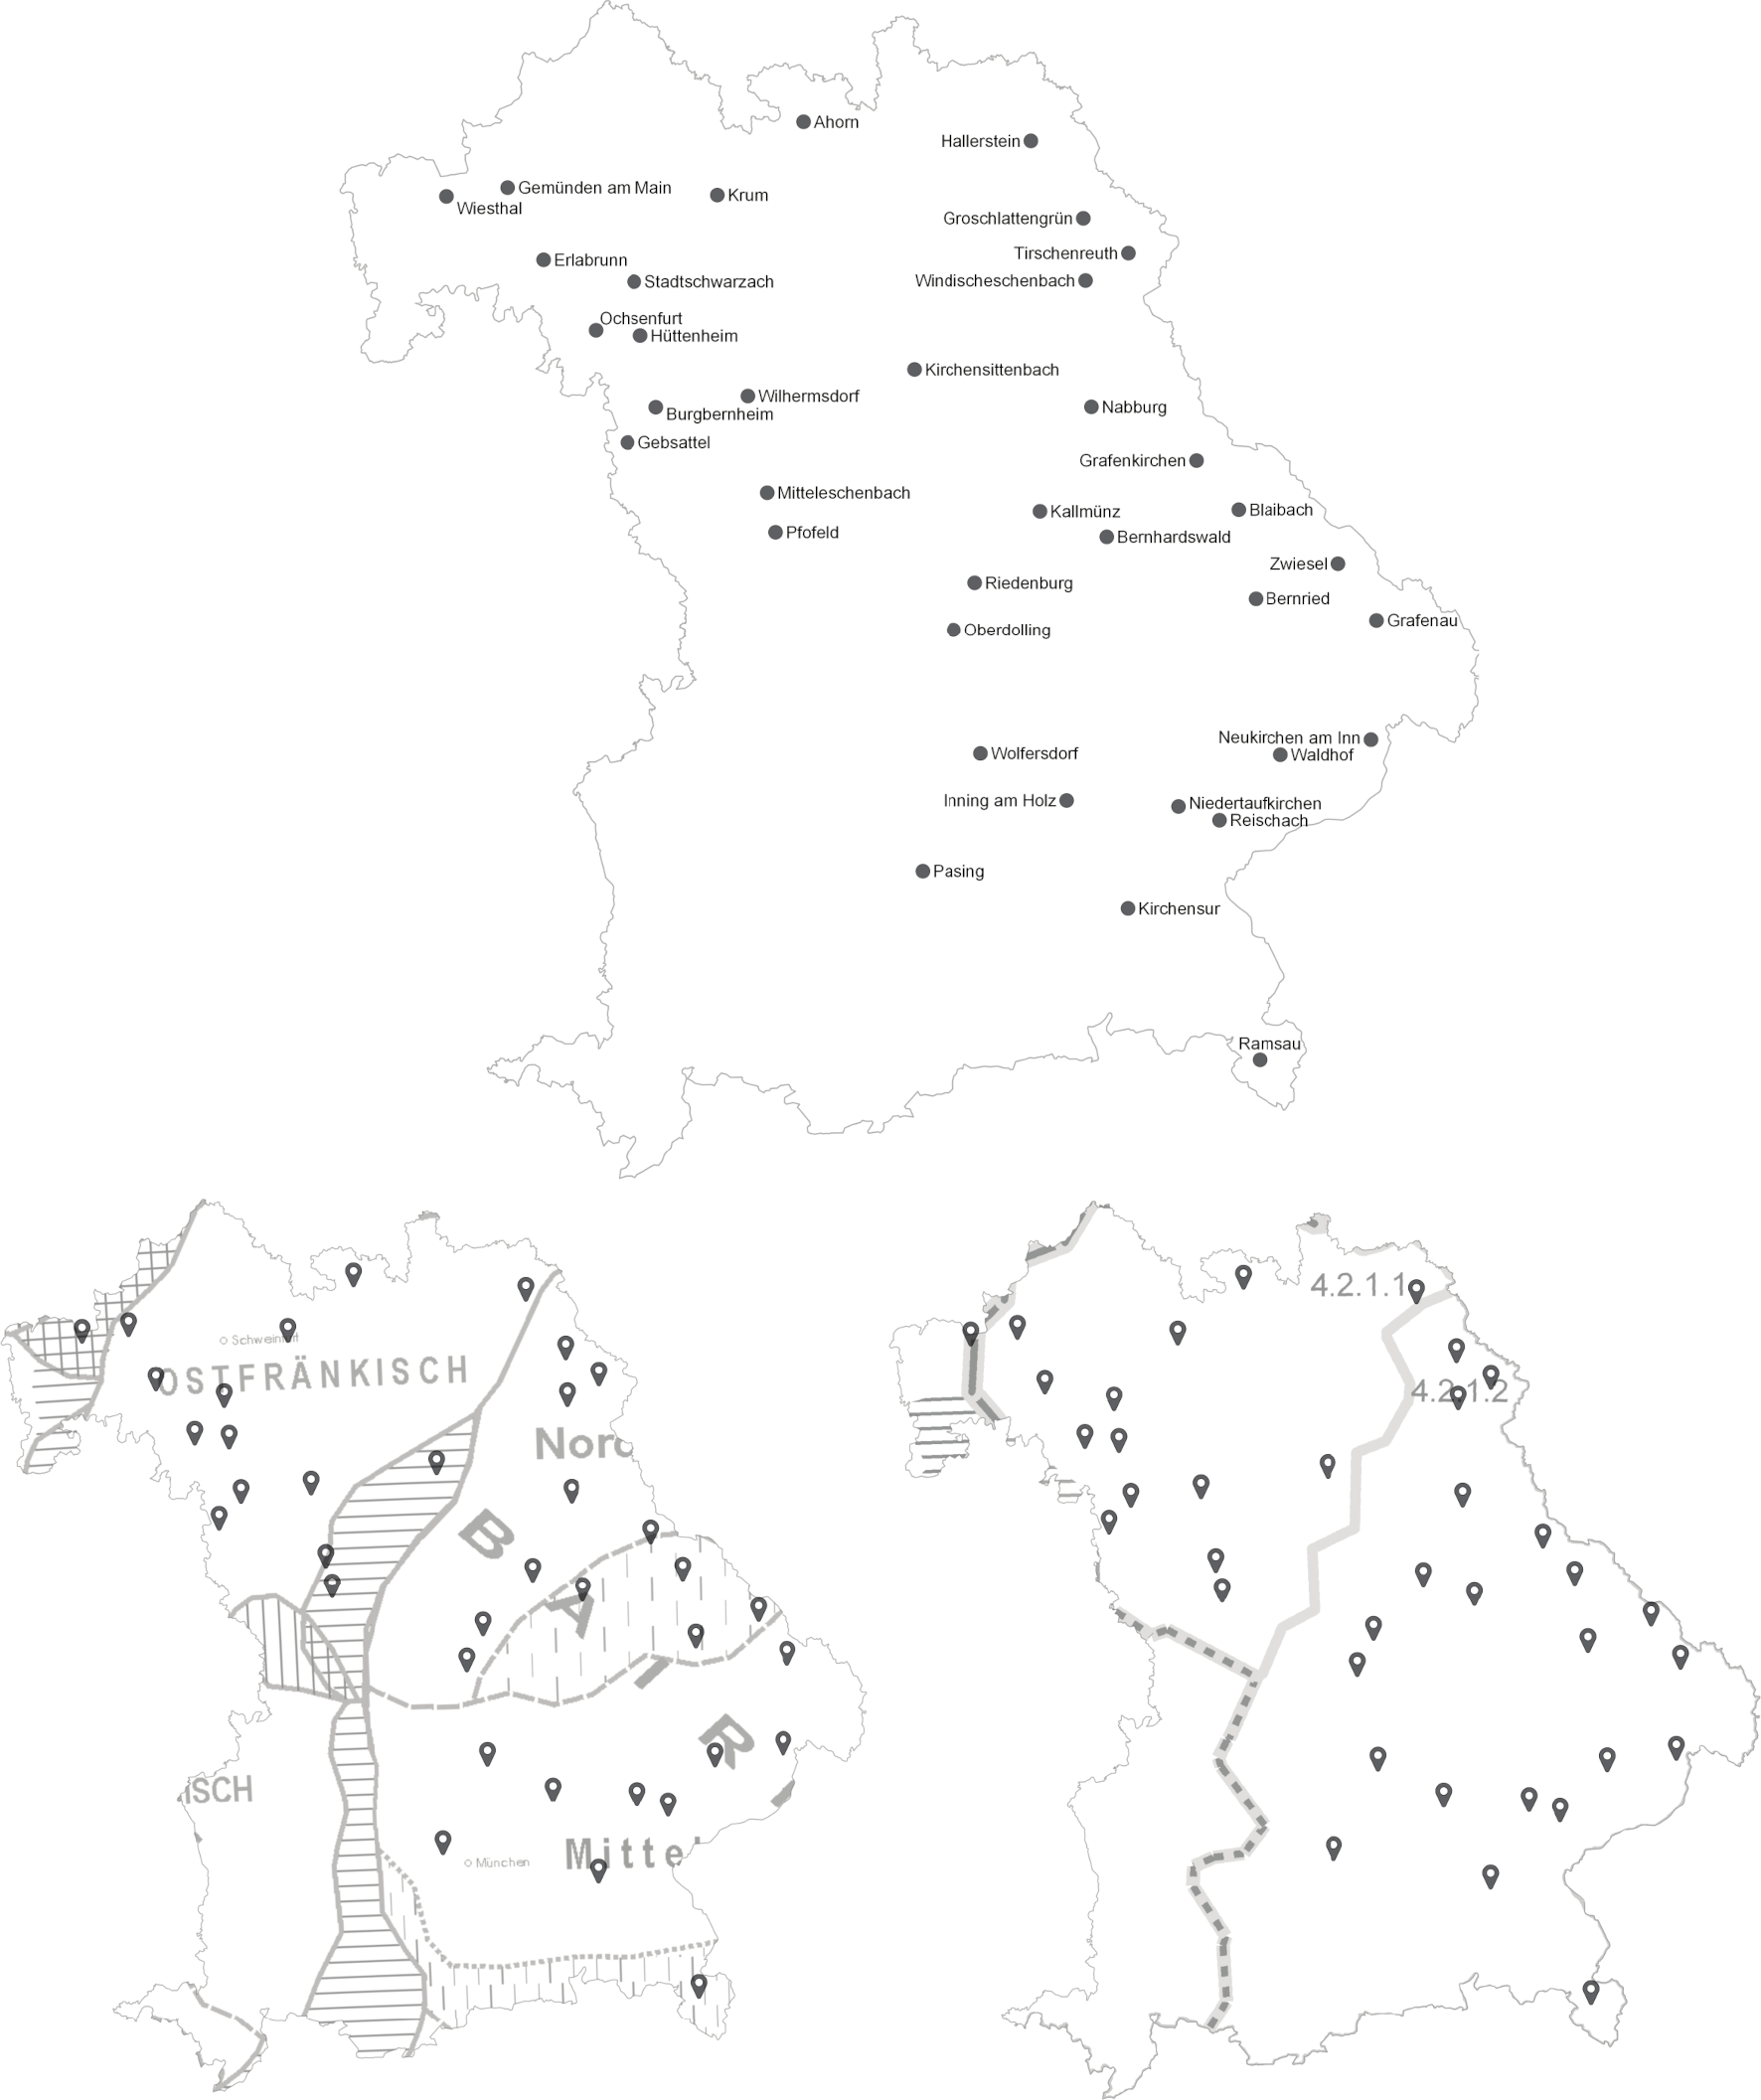
\includegraphics[width=\textwidth]{figures/Karte1.png}
\caption{Tiefenbohrungspunkte sowie Ortspunkte mit den Dialektgliederungen von \citet[Karte 47.4, unten links]{Wiesinger1983b} und \citet[194, unten rechts]{Lameli2013}}
\label{map:1}
\end{map}

Die Abgrenzung des Ofr. und dessen spezifischer Dialektmerkmale wurden in der Literatur unterschiedlich bewertet (vgl. den Überblick in \citealt{Harnisch2019} und \citealt{Rowley1990a}). Anhand einer
Analyse von Similaritätsrelationen von obd. Referenzorten\footnote{Die obd. Referenzorte sind Kitzingen (Ofr.), Dachau (Mittelbair.), Reutlingen (Schwäbisch).} belegt \citet[168ff.]{Lameli2013} zum einen, dass es „eine starke Anbindung“ des Ofr. an das Bair. gibt, „die umgekehrt nicht gleichermaßen vorliegt“. Zum anderen weisen die Ähnlichkeitswerte des Schwäbischen und deren im Vergleich zu den anderen obd. Dialekträumen weniger große Reichweite darauf hin, dass eine Grobunterteilung des Oberdeutschen in West- und Ostoberdeutsch sinnvoll ist.\footnote{Dieser Befund wird gestützt durch die Analyse von Phylogrammclustern, die eine enge Verbindung zwischen dem ofr. und bair. (d.\,h. oobd.) Sprachraum gegenüber einem alem. und schwäb. (westoberdeutschen) Sprachraum visualisieren (\citealt[187f.]{Lameli2013}).} In der Analyse \citegen[169f.]{Lameli2013} zeigt Kitzingen als ofr. Referenzort „eine klar oberdeutsche Prägung“, wenngleich der Similaritätsvergleich auch Ähnlichkeiten zu den mitteldeutschen Dialekten aufzeigt und damit die Stellung des Ofr. zwischen mittel- und oberdeutschem Sprachraum bestätigt. Zugleich bildet das Ähnlichkeitsprofil von Kitzingen eine Binnendifferenzierung des Ostfränkischen in Unter- und Oberofr. durch die sogenannte Steigerwaldschranke ab, wobei das Oberofr. wiederum ein Übergangsgebiet zum Bair. darstellt (\citealt[203, FN 274]{Lameli2013}). Für den bair. Dialektraum stellt \citet[171]{Lameli2013} fest, dass er in seiner räumlichen Ausdehnung das größte und hinsichtlich der Similaritätswerte einheitlichste Areal unter den deutschen Dialekten bildet. Die Similaritätsmuster illustrieren zugleich „nachdrücklich die signifikante Mittelstellung“ des Nordbair. zwischen dem ofr. und bair. UG (\citealt[173]{Lameli2013}, vgl. \citealt[288--290]{Koch2019} und \citealt[171--174]{Rowley1997}).\largerpage[2]

Eines der Untersuchungsziele besteht in der Beschreibung der horizontalen Variationsdimension der Pluralmarkierung: Sind bestimmte Pluralkodierungsverfahren dialekt(raum)spezifisch und arealbildend? Daneben soll untersucht werden, ob und inwiefern phonologische Voraussetzungen die Flexionsmorphologie bedingen, also in welchem Maße das Pluralmarkerinventar durch das Phoneminventar und/oder durch phonologische Prozesse gesteuert ist. Die Auswahl der Tiefenbohrungspunkte musste daher einem doppelten Kriterium entsprechen. Zum einen sollen sie die verschiedenen Dialekträume im UG abbilden, zum anderen sollen die phonologischen Voraussetzungen so variant sein, dass sie einen Vergleich von dialektalen Markierungsstrategien und phonologischen Variablen ermöglichen. Ausgewählt wurden Ortspunkte, für die in jedem Falle ein Wenker-Bogen und nach Möglichkeit auch eine Orts- oder Landschaftsgrammatik vorliegt, sodass nicht nur der synchrone Formenbestand der Pluralmarker, sondern auch eine Kurzzeitdiachronie untersucht werden konnte. Um sicherzustellen, dass eine mögliche Raumbildung nicht durch zufällige Unterschiede im erfassten Datenmaterial, sondern aus einer inhärenten Systematik abzuleiten ist, wurden immer mehrere, räumlich nahe Ortspunkte definiert („Cluster“). Idealerweise sollten sowohl vor dem Hintergrund einzelner Arbeitsgebiete der BSA-Teilprojekte als auch für die einzelnen Dialekträume im UG eine ausgeglichene Menge solcher Tiefenbohrungspunkte definiert werden.

Für die Auswahl der Ortspunkte ermöglichten vorhandene Dialekteinteilungen (\citealt{Wiesinger1983b}, \citealt{Lameli2013}) einen ersten Zugang. Methodisch besteht dabei die Gefahr eines Zirkelschlusses, da Dialekteinteilungen primär auf phonologischen neben morphologischen Varianten basieren und die ausgewählten Tiefenbohrungspunkte diese Befunde im schlimmsten Fall nur reproduzieren. Dies kann insofern relativiert werden, als jede Dialekteinteilung das Ergebnis einer qualitativen Kontrastierung bestimmter Kriterien (d.\,h. prototypischer Varianten) und damit das Ergebnis einer Reduzierung der arealtypologischen Komplexität der sprachlichen Wirklichkeit ist \citep[8]{Lameli2013}. So basiert die strukturelle Dialekteinteilung \citegen{Wiesinger1983b} vor allem auf prototypischen phonologischen neben (flexions-)morphologischen Kriterien, die als Einzelvarianten und in Form einer Zusammenfassung zu Variantenbündeln die Grundlage dieser Dialektklassifikation sind \citep[812--814]{Wiesinger1983b}. Eine tiefergehende Analyse der nominalen Flexionsformen geht weit über diese ausgewählten Varianten hinaus und ergänzt diese vielmehr, als dass sie nur reproduziert werden.\largerpage

Ein Spezifikum und großer Vorteil der Wiesinger-Einteilung ist die Unterscheidung von Kern- und Übergangsgebieten, die aus der Einteilungskarte hervorgeht (\citealt[830f. und Karte 47.4]{Wiesinger1983b}; vgl. \citealt[188--189]{Lameli2019}). In der vorliegenden Untersuchung wurden neben den Kern- auch Übergangs- und Randgebiete berücksichtigt: Unterostfränkisch (inklusive ofr.-hess. Übergangsgebiet), Oberostfränkisch, nördliches Nordbairisch (inklusive ofr.-nordbair. Über"-gangs"-ge"-biet), südliches Nordbairisch und nordbair.-mittelbair. Übergangsgebiet, Mittelbair. (inklusive mittelbair.-südbair. Übergangsgebiet). Aus dem Pool möglicher Tiefenbohrungspunkte (d.\,h. Ortspunkten, die sowohl Wenker- als auch BSA-Erhebungsorte waren) wurden in einem nächsten Schritt Ortspunkte mit möglichst differenten phonologischen Profilen gewählt. Hierfür wurden die Karten des \textit{Deutschen Sprachatlas} („Wenker-Atlas“, \citealt{WA}), die publizierten BSA-Bände sowie Dialektgrammatiken und -darstellungen hinsichtlich verschiedener phonologischer Prozesse gesichtet (\tabref{tab:12}). Neben diesen phonologischen Variablen bildeten potenzielle Unterschiede der Numerusmorphologie im intervarietären Vergleich oder im Vergleich von Standard und Dialekt ein weiteres Auswahlkriterium.


\mapref{map:1} zeigt die 37 definierten Tiefenbohrungspunkte. Für den Westen des Ofr. und auch für die nordbair. Cluster wurde jeweils ein dichteres Ortsnetz gewählt, da hier Isoglossen verschiedener Variablen des Vokalismus und der Reduktionssilbe verlaufen (vgl. \citealt[399]{Rowley1990a}). Die Durchsicht vorhandener Sprachkarten zu den einzelnen Phänomenen bestätigt dagegen \citegen[171]{Lameli2013} Befund, dass das Mittelbair. innerhalb des bair. Dialektraum ein sprachlich konsistentes Gebiet bildet, weswegen hier ein weniger dichtes Ortsnetz definiert wurde.\largerpage

\begin{table}
\caption{Phonologische und flexionsmorphologische Kriterien sowie Binnengliederung des UGs (vgl. \citealt[4--5]{Rowley1997})\label{tab:12}}

\begin{subtable}{\textwidth}
\caption{Vokalqualität I\label{tab:12a}}
\small
\begin{tabularx}{\textwidth}{>{\raggedright\arraybackslash}p{.2\textwidth}QQ}
\lsptoprule

\multicolumn{2}{p{.45\textwidth}}{Auswahlkriterien der (historischen) Phonologie und Flexions\-morphologie} & Binnengliederung des Untersuchungs\-gebiets: Dialektraum und Ortsdialekte\\
\midrule
Umlaut\slash Nicht-Eintreten des Umlauts & Umlaut/Nicht-Umlaut bei mhd. \textit{u}/\textit{ü} (vgl. \citealt{Hinderling2004}, \citealt[159ff.]{SNOB1}) & Bair. Cluster, nordöstliches Ofr. (Ahorn, Hallerstein)\\
\tablevspace
Hebung\slash Senkung & Hebung und z.\,T. Diphthongierung von mhd. \textit{e}, \textit{ö}, \textit{o} in Dehnung (\citealt{Gütter1971}: Karte 3/4, \citealt{Rowley1997}: 73--74/Karte 15) & nördliches Nordbair. (Gro\-schlat\-ten\-grün, Windischeschenbach, Tir\-schen\-reuth) und Coburger, Nürnberger und Weißenburger Raum (Ahorn, Kirchensittenbach, Mittelschenbach, Pfofeld)\\
\tablevspace
& Senkung von mhd. \textit{i} & Wiesthal\\
\tablevspace
& Senkung\slash Zentralisierung von mhd. \textit{ë} (\citealt{WA}-Karten 405 „Berge“, 524 „Felde“) & Hüttenheim, Stadtschwarzach\\
\tablevspace
Rundung\slash Entrundung & Rundung von Palatalvokalen (vgl. \citealt[1103]{Wiesinger1983e}, \citealt{WA}-Karte 465 „Häuser“) & ofr.-hess.-hennebergisches Gebiet (unterofr. Cluster, ofr. Ahorn)\\
\tablevspace
& Entrundung von Palatalvokalen (\citealt{WA}-Karte 465 „Häuser“) & Nürnberger Raum, Nord- und Mittelbair.\\
\lspbottomrule
\end{tabularx}
\end{subtable}
\end{table}


\begin{table}
\ContinuedFloat
\caption{Phonologische und flexionsmorphologische Kriterien sowie Binnengliederung des UGs (vgl. \citealt[4--5]{Rowley1997})}

\begin{subtable}{\textwidth}
\caption{Vokalqualität II}
\label{tab:12b}
\small
\begin{tabularx}{\textwidth}{>{\raggedright\arraybackslash}p{.25\textwidth}QQ}
\lsptoprule

\multicolumn{2}{p{.45\textwidth}}{Auswahlkriterien der (historischen) Phonologie und Flexions\-morphologie} & Binnengliederung des Untersuchungs\-gebiets: Dialektraum und Ortsdialekte\\
\midrule
Monophthongierung/ Diphthongier\-ung & Monophthongierung der Diphthongierungsprodukte bei mhd. \textit{î}, \textit{û}, \textit{iu} (sogenannte „tertiäre Monophthonge“, vgl. \citealt{Wildfeuer2004}, \citealt{WA}-Karten 51 „Eis“, 373 „Hause“, 465 „Häuser“) & südöstliches Nordbair., nordbair-mittelbair. Übergangsgebiet (Bernried, Blaibach, Grafenkirchen)\\
\tablevspace
& Monophthongierung von mhd. \textit{öu} (vgl. \citealt{WA}-Karte 380 „Apfelbäumchen“) & ofr. und mittelbair. Cluster \\
\tablevspace
& Monophthongierung von mhd. \textit{ei} (vgl. \citealt{WA}-Karten 96 „Eier“, 443 „Seife“) & Ofr., bei \textit{Ei} nur im unterofr. Cluster (Erlabrunn, Gemünden, Hüttenheim, Ochsenfurt, Wiesthal)\\
\tablevspace
& Vokalwechsel von mhd. \textit{ei} in historischen Ein- und Mehrsilbern & Nordbair. und nordbair.-mittelbair. Über\-gangsgebiet, nordöstl. Mittelbair.\\
\lspbottomrule
\end{tabularx}
\end{subtable}
\end{table}


\begin{table}
\ContinuedFloat
\caption{Phonologische und flexionsmorphologische Kriterien sowie Binnengliederung des UGs (vgl. \citealt[4--5]{Rowley1997})}

\begin{subtable}{\textwidth}
\caption{Konsonantismus}
\label{tab:12c}
\small
\begin{tabularx}{\textwidth}{>{\raggedright\arraybackslash}p{.25\textwidth}QQ}
\lsptoprule

\multicolumn{2}{p{.45\textwidth}}{Auswahlkriterien der (historischen) Phonologie und Flexions\-morphologie} & Binnengliederung des Untersuchungs\-gebiets: Dialektraum und Ortsdialekte\\
\midrule
Fortis-Lenis-Opposition & Aufhebung der Fortis/Lenis-Opposition in allen Positionen & Ofr.\\
\tablevspace
& „Bair. Silbengesetz“ & Nord- und Mittelbair.\\
\tablevspace
Liquidvokalisierung & Vokalisierung von /l/ zu [i] (\citealt{Gütter1971}: Karte 6) & mittelbair. Cluster, nordbair.-mittelbair. Übergangsgebiet\\
\lspbottomrule
\end{tabularx}
\end{subtable}
\end{table}

\begin{table}
\ContinuedFloat
\caption{Phonologische und flexionsmorphologische Kriterien sowie Binnengliederung des UGs (vgl. \citealt[4--5]{Rowley1997})}

\begin{subtable}{\textwidth}
\caption{Reduktionssilben}
\label{tab:12d}
\small
\begin{tabularx}{\textwidth}{>{\raggedright\arraybackslash}p{.2\textwidth}QQ}
\lsptoprule

\multicolumn{2}{p{.45\textwidth}}{Auswahlkriterien der (historischen) Phonologie und Flexions\-morphologie} & Binnengliederung des Untersuchungs\-gebiets: Dialektraum und Ortsdialekte\\
\midrule
Schwa-Erhalt\slash Apokope & Schwa-Erhalt bei \textit{Gänse}, \textit{Berge} (\citealt{WA}-Karten 188, 406) & Hallerstein, Pfofeld, Wiesthal\\
\tablevspace
vokalische Realisierung des Nasalsuffixes & Vokalische Realisierung des Nasalsuffixes in allen Positionen und phonologischen Umgebungen (\citealt{WA}-Karten 444 „Seife“, 492 „Bauern“, 495 „Ochsen“, 546 „hinten“) & „Vokalisierungsstreifen“ im westlichen Ofr. (Erlabrunn, Gebsattel, Gemünden, Ochsenfurt)\\
\tablevspace
& Vokalisierung des Nasalsuffixes in Abhängigkeit von der phonologischen Umgebung & mittleres und östl. Ofr., Nord- und Mittelbair. \\
\lspbottomrule
\end{tabularx}
\end{subtable}
\end{table}

\begin{table}
\ContinuedFloat
\caption{Phonologische und flexionsmorphologische Kriterien sowie Binnengliederung des UGs (vgl. \citealt[4--5]{Rowley1997})}

\begin{subtable}{\textwidth}
\caption{Nominale Flexionsmorphologie}
\label{tab:12e}
\small
\begin{tabularx}{\textwidth}{>{\raggedright\arraybackslash}p{.2\textwidth}QQ}
\lsptoprule

\multicolumn{2}{p{.45\textwidth}}{Auswahlkriterien der (historischen) Phonologie und Flexions\-morphologie} & Binnengliederung des Untersuchungs\-gebiets: Dialektraum und Ortsdialekte\\
\midrule
einzelne Phänomene der Formenbildung & subtraktive Pluralmarkierung (vgl. \citealt{Köhler1934}) & Gemünden am Main, Wiesthal\\
\tablevspace
& keine Pluralmarkierung durch Quantitätskontraste (\citealt{SMF7}: Karte 21) & Wilhermsdorf\\
\tablevspace
& schwache Pluralmarkierung bei \textit{Berge} (\citealt{WA}-Karte 406) & Bernried, Blaibach, Waldhof\\
\tablevspace
& Singularstammbildung der historisch schwachen Feminina: keine \textit{n}{}-Erweiterung, sondern Apokope (\citealt{WA}-Karte 444 „Seife“) & südbair.-mittelbair. Übergangsgebiet (Ramsau bei Berchtesgaden)\\
\tablevspace
& erweitertes Nasalsuffix im Dativ Plural (\citealt{SMF7}: Karte 24) & Mitteleschenbach\\
\tablevspace
& kein Nasalsuffix im Dativ Plural (\citealt{SMF7}: Karte 24) & westliches Ofr. (Burgbernheim, Gebsattel)\\
\lspbottomrule
\end{tabularx}
\end{subtable}
\end{table}

\clearpage
\section{Die Materialbasis}\label{sec:6.2}
\begin{sloppypar}
Die Datenbasis besteht aus drei verschiedenen Quellentypen: als primäre Datenbasis die Erhebungsdaten des \textit{Bayerischen Sprachatlas} und die Sprachatlanten der einzelnen Teilprojekte (\sectref{sec:6.2.1}), daneben die Daten der Wenker-Erhebungen und die Karten des \textit{Sprachatlas des Deutschen Reiches} (\sectref{sec:6.2.2}) und diverse grammatische Beschreibungen der untersuchten Dialekte (insbesondere Orts- und Landschaftsmonografien, aber auch Zeitschriftenbeiträge oder nicht publizierte Qualifikationsarbeiten, vgl. \sectref{sec:6.2.3}). Die Datenbasis ist damit ausgesprochen heterogen in ihrer methodischen Ausrichtung und Darstellung, bezieht sich aber jeweils auf den Basisdialekt als am weitesten vom Standard entfernte Varietät.
\end{sloppypar}

Indem die vorliegende Arbeit das vorhandene Erhebungsmaterial des \textit{Bayerischen Sprachatlas} und historisches Datenmaterial aus Orts- und Landschaftsgrammatiken verwendet, ist sie an die abgefragten bzw. behandelten, meist isolierten Flexionsformen dieser Quellen und an einen sehr spezifischen Ausschnitt meist landwirtschaftlicher Lexik gebunden. Jüngere Arbeiten haben indes gezeigt, dass die Auswertung von Dialektgrammatiken als Datenquellen für morphologische Fragestellungen ein sinnvolles und gewinnbringendes Unterfangen darstellt (vgl. \citealt{Birkenes2014, Fischer2018, Fischer2019}). Gleichzeitig ist es durch die digitale Verfügbarkeit beinahe des gesamten Abfragematerials der Teilprojekte des \textit{Bayerischen Sprachatlas} und der Wenker-Materialien möglich, Datenmaterial und Karten zu den einzelnen Teilsystemen der Grammatik für die Tiefenbohrungspunkte oder ganze Dialekträume zu vergleichen und systematisch in die Datenauswertung einzubeziehen.

Eine methodische Schwierigkeit bei der Nutzung vorhandener Dialektdaten zu einer flexionsmorphologischen Fragestellung besteht nach wie vor darin, dass in dem zur Verfügung stehenden Datenmaterial kaum vollständige Flexionsparadigmen belegt sind, während für den Bereich der Phonologie -- dies entspricht dem primären Erkenntnisinteresse der traditionellen Dialektologie -- das gesamte phonologische System ausgehend vom mhd. Protosystem erhoben wurde. In der Nominalflexion wurden meist nur einzelne Paradigmenstellen abgefragt, im Falle des BSA beispielsweise Nominativ Singular und Plural, z.\,T. Akkusativ \mbox{und}\slash oder Dativ Singular und\slash oder Plural (vgl. \citealt[814]{Rabanus2010}). Der Vorteil der Daten des \textit{Bayerischen Sprachatlas} besteht in erster Linie darin, dass für das gesamte Untersuchungsgebiet ein weitgehend einheitliches Fragebuch verwendet wurde. Für Einzellexeme ist die Datenlage damit vergleichsweise gut; Nominalphrasen wurden noch selektiver erhoben und z.\,T. nicht vollständig transkribiert, weswegen sie im Rahmen der Untersuchung nur für die syntaktische Einheit Definitartikel und Substantiv systematisch aufbereitet wurden.

Tonkorpora (zum Beispiel das Zwirner-Korpus im \textit{Archiv für Gesprochenes Deutsch} oder die Tonaufnahmen der BSA-Teilprojekte, die bei den Explorationen aufgenommen wurden) wurden in dieser Untersuchung nicht berücksichtigt. Spontansprachliches Material ist für eine flexionsmorphologische Untersuchung zwar wünschenswert (v.\,a. dann, wenn Synkretismen vorliegen und die Sprecher Ambiguitäten auflösen müssen) und auch reich an flexivischen Formen, jedoch ist die Auswertung ausgesprochen aufwendig und bei freien Dialogen eine entsprechend große Menge an Datenmaterial nötig, wenn ein ähnlich vergleichbares Korpus aufgebaut werden soll, wie es dieser Arbeit zugrunde liegt (vgl. hierzu auch \citealt[37]{Birkenes2014}, \citealt[39]{SchmidtEtAl2019}).

\subsection{Der \textit{Bayerische Sprachatlas} und seine Teilprojekte}
\label{sec:6.2.1}

\begin{quote}
Wir sehen die Fertigstellung der Bände nicht als das Ende, sondern als den entscheidenden Schritt für die weitere dialektologische Arbeit an. \\\hbox{}\hfill\hbox{(\citealt[7]{SNiB3})\footnote{Die Kurzzitation der publizierten Bände des \textit{Bayerischen Sprachatlas} nennt jeweils Teilprojekt und Bandnummer (z~B. SNiB 3 für \textit{Sprachatlas von Niederbayern}, Band 3), eine Aufschlüsselung der zitierten Bände findet sich im Literaturverzeichnis.}}
\end{quote}

Der \textit{Bayerische Sprachatlas} steht in der Tradition von Georg Wenkers \textit{Sprachatlas des Deutschen Reichs}, setzt zugleich die Methodik des \textit{Sprachatlas der Deutschen Schweiz} von Rudolf Hotzenköcherle fort und knüpft damit an die Methodik der Sprachatlanten der sogenannten zweiten Generation: die direkte Befragung der ältesten ortsansässigen Informanten (\textit{non-mobile, old, rural males} und \textit{females}, vgl. \citealt[29]{ChambersTrudgill2009}) durch geschulte Exploratoren, um so einzig die horizontale, d.\,h. diatopische Dimension von Variation zu erheben. Ziel der direkten Erhebungen im Rahmen der BSA-Teilprojekte war es, „den jeweils ältesten noch erreichbaren Sprachstand zu Papier zu bringen“ (\citealt[25]{SBS1}). Die Einzelinformation der befragten NORMs und NORFs und ihre metasprachliche Kompetenz stehen damit repräsentativ für den jeweiligen Ortsdialekt (vgl. \citealt[500--501]{König2010}). Als Ergebnis dieser Operationalisierung der repräsentativen Einzelinformation durch NORMs/NORFs arbeitet die traditionelle Dialektologie mit einer sehr spezifischen Form von Sprachdaten: Die erhobene Varietät, der Basisdialekt (auch Grunddialekt), ist, wie \citet[24f.]{Auer2010} betont, kein der Forschung „vorgängiges und von ihr unabhängiges Objekt der sprachlichen Wirklichkeit“, sondern „ein dem Alltag fremdes, in der Situation der Erhebung entstehendes Objekt“.\footnote{Auch während der BSA-Erhebungen war man sich darüber „bewußt, daß die Auskünfte der Gewährsleute über ihre Sprachverwendung nicht in jedem Fall mit einer aufgrund von Langzeitbeobachtung gewonnen Ortsnorm übereinstimmen müssen“ (\citealt[26]{SBS1}).} Das Datenmaterial der traditionellen Dialektologie ist folglich Ergebnis eines „Konstitutionsprozesses“ \citep{Auer2010}. Der erhobene (intendierte) Basisdialekt muss als Konstrukt zur Datenerhebung verstanden werden (vgl. \citealt[502]{König2010}): „Der Explorator verwandelt die Antworten der Gewährspersonen also in Daten; das Konstrukt Grunddialekt wird durch ihn genauso geformt wie durch den Informanten“ \citep[34]{Auer2010}. Durch das Forschungsziel und das methodische Vorgehen der BSA-Projekte ergibt sich für die entstandenen Sprachatlanten „eine Position zwischen historischer und rezenter Sprachwissenschaft“ (\citealt[37]{SMF1}), das Ergebnis ist die Dokumentation einer Sprachschicht, „die einerseits bereits historisch ist, andererseits aber noch direkt erhoben werden kann“ (ebd.).

Die Arbeitsgebiete der Regionalprojekte des \textit{Bayerischen Sprachatlas} -- mit Ausnahme des \textit{Sprachatlas von Bayerisch Schwaben}, dessen Arbeitsgebiet das gesamte Areal des Alemannischen und Schwäbischen in Bayern abdeckt -- entsprechen den Regierungsbezirken Bayerns (\tabref{tab:13}). Um die jeweilige Größe des Erhebungsgebietes abschätzen zu können, wurden als Referenz die Anzahl der Planquadrate angegeben (mit einer Kantenlänge von 7 km, geplant war eine Ortsaufnahme pro Planquadrat, vgl. \citealt[21]{Klepsch2013}).

\begin{table}
\begin{tabularx}{\textwidth}{QQll}
\lsptoprule
Teilprojekt & Untersuchungsgebiet & \makecell[tl]{Plan-\\quadrate} & \makecell[tl]{Erhebungs-\\zeitraum}\\
\midrule
Sprachatlas von Mittelfranken

(SMF) & Regierungsbezirk

Mittelfranken & 155 & 1991--1998\\
\tablevspace
Sprachatlas von Unterfranken

(SUF) & Regierungsbezirk

Unterfranken & 180 & 1991--1996\\
\tablevspace
Sprachatlas von Nordostbayern

(SNOB) & Regierungsbezirke

Oberfranken und Oberpfalz & 360 & 1981--1999\\
\tablevspace
Sprachatlas von Niederbayern

(SNiB) & Regierungsbezirk

Niederbayern & 240 & 1991--1998\\
\tablevspace
Sprachatlas von Oberbayern

(SOB) & Regierungsbezirk Oberbayern & 320 & 1991--1998\\
\lspbottomrule
\end{tabularx}
\caption{Die in der Untersuchung berücksichtigten Teilprojekte des \textit{Bayerischen Sprachatlas}}
\label{tab:13}
\end{table}

Die einzelnen Teilprojekte arbeiten mit einem gemeinsamen Fragebuch von rund 2.800 Fragen. Um die Vergleichbarkeit der Teilprojekte zu gewähren, wurde der Aufbau des Fragebuchs nicht verändert, aber um mögliche regionalspezifische Aspekte ergänzt (z.\,B. zum Hopfen- und Weinanbau, mit einem Anteil von bis zu 10\,\% projektspezifischer Fragen am Fragebuch insgesamt, vgl. \citealt[6]{Munske2015}). Die Fragebücher waren nach außersprachlichen Themenbereichen („Das Vieh und seine Pflege“, „Ackerbau“, „Boden und Flur“ etc.) gegliedert und subsumierten darunter sowohl Fragen zur spezifischen Lexik als auch zu sprachstrukturellen Aspekten. Die Exploratorinnen und Exploratoren arbeiteten den vorgedruckten Fragekatalog mit den Gewährspersonen durch, wobei das Gespräch möglichst frei gestaltet sein sollte (vgl. \citealt[31]{SMF1}). Ziel der semasiologischen Fragestellungen im Fragebuch war es, „Aufschluß über die Strukturen der Mundart“ zu erhalten und schließlich mithilfe des dokumentierten Sprachmaterials jeder Ortsaufnahme eine Ortsgrammatik anfertigen zu können (\citealt[31]{SMF1}).


\begin{table}
\small
\begin{tabularx}{\textwidth}{lQcccccccc}
\lsptoprule

& Band & Genus & \multicolumn{2}{c}{ Flexion} & \multicolumn{2}{c}{Nominalphrase} & \multicolumn{3}{c}{ Wortbildung}\\
\cmidrule(lr){4-5}\cmidrule(lr){6-7}\cmidrule(lr){8-10}
&  &  & Num. & Kas. & Art.\slash Pron. & Adj. & Der. & Dim. & Mov.\\
\midrule
SBS & 9.1, 9.2 &  & x & x & x & x & x & x & x\\
SMF & 7 &  & x & x &  &  & x & x & x\\
SUF & 3 &  & x & x & x & x &  & x & x\\
SNiB & 7 & x & x &  &  &  &  & x & \\
SOB & 3 & x & x &  & x &  &  & x & \\
SNOB & \multicolumn{9}{l}{ noch nicht erschienen}\\
\lspbottomrule
\end{tabularx}
\caption{Überblick der behandelten Themen zur Nominalmorphologie in den BSA-Teilbänden (vgl. \citealt[8--9]{Munske2015}). Wortbildungen: „Der.“: Deri\-va\-tion, „Dim.“: Dimi\-nu\-tion, „Mov.“: Mo\-vie\-rung}
\label{tab:14}
\end{table}

Diesem Forschungsziel entsprechend bilden die BSA-Fragebücher und im Ergebnis die publizierten Bände alle Sprachebenen ab (zum Teil mit regionalen Schwerpunkten wie dem Syntax-Programm des SNiB). Doch auch in den Teilprojekten des \textit{Bayerischen Sprachatlas} (wie auch in anderen Sprachatlasprojekten) bildete die Phonologie (neben der Lexik) den zentralen Interessensbereich, was sich bereits im Fragebuch, vor allem aber an Umfang und Anzahl der publizierten Bände ablesen lässt. Die Phonologie ist auf mehrere Bände getrennt nach Lang- und Kurzvokalismus sowie Konsonantismus aufgeteilt, während die Morphologie zumeist einen Band, z.\,T. aber auch nur einen Halbband umfasst (nur im Fall des SUF und des SBS sind es zwei). Und auch ein Blick in die Inhaltsverzeichnisse der jeweiligen Morphologie(teil)bände zeigt, dass das Ziel respektive Arbeitsprinzip der BSA-Teilprojekte, nämlich die Abbildung der „sprachgeographisch relevanten, d.h. raumbildenden Erscheinungen“ \citep[5]{Munske2015}, dazu führte, dass die (nominale) Flexionsmorphologie als Flexions\textit{system} nur punktuell behandelt wurde. Kartiert wurden v.\,a. Flexionsformen einzelner Lexeme (nach Genus und Pluralmarkierungsverfahren sortiert, daneben ausgewählte Aspekte der Flexion der Substantivbegleiter und der Wortbildung). Da die Auswahl und die Art der Darstellung den jeweiligen Teilprojekten oblagen, sind für das gesamte Untersuchungsgebiet trotz des weitestgehend einheitlichen Fragebuchs nicht dieselben und vor allem nicht sämtliche Lexeme und Phänomenbereiche der Nominalflexion kartiert. Eine flächendeckende Auswertung des gesamten Rohmaterials ist -- dies illustriert \tabref{tab:14} -- auch nach Erscheinen der Bände des \textit{Bayerischen Sprachatlas} ein Desiderat.

Für die vorliegende Untersuchung wurden die nicht-typisierten Rohdaten der BSA-Teilprojekte zur Flexion des Substantivs aufbereitet und ausgewertet (siehe Anhang). Diese sind über die \textit{Bayerische Dialektdatenbank} \textit{BayDat} in einer online verfügbaren Datenbank zugänglich (vgl. \sectref{sec:6.3.1.1}). Eine Untersuchung zur Nominalflexion kann dabei eine andere Zielsetzung und Vorgehensweise verfolgen als ein Sprachatlas: Während es hier vor allem um die Erfassung des Systems geht, bestand das Ziel da eher in der Dokumentation ausgewählter Varianten. Dabei sind die nicht-typisierten Rohdaten ausgesprochen geeignet, um sprachliche Strukturen zu untersuchen und so „den bisherigen sprachgeographischen Schwerpunkt zugunsten eines sprachsystematischen zu verschieben“ (\citealt[22]{Munske2015}, vgl. \citealt[70]{Kretzschmar2018}). So werden -- anders als in einzelnen Morphologiebänden des BSA -- phonetisch-phonologische Varianten weniger stark in den Vordergrund gestellt, die Daten noch stärker abstrahiert und nach einzelnen Konditionierungsfaktoren der Pluralallomorphie und Deklinationsklassenzusammensetzung untersucht. Zugleich kann eine Analyse der Flexion eines Ortsdialekts kaum losgelöst vom grammatischen Gesamtsystem erfolgen (vgl. \citealt[36]{Schmuck2014}). Die publizierten BSA-Bände (insbesondere jene zur Phonologie und zur Syntax), ihre Analysen und Typisierungen dienen im Folgenden daher als zusätzliche Referenz.

Im Rahmen der Untersuchung wurden die transkribierten Belege der direkten Befragungen der Gewährspersonen ausgewertet, d.\,h. Flexionsformen (Substantive, Nominalphrasen sowie vereinzelte Sätze), die von den Gewährspersonen innerhalb einer spezifischen Erhebungssituation realisiert wurden. Abgefragt wurden isolierte Flexionsformen, syntaktische Strukturen und Verwendungskontexte, die durch die Exploratoren vorgegeben und von den Gewährspersonen in den Ortsdialekt übersetzt wurden (vgl. \citealt[23]{Klepsch2013}).\footnote{Im \textit{Sprachatlas von Mittelfranken} (als exemplarisches Beispiel für die BSA-Fragebücher insgesamt) behandeln von den insgesamt 2.541 semasiologischen Fragen des SMF-Fragebuchs die meisten die Grundform, im nominalen Bereich also den Nom.Sg. (vgl. \citealt[24]{Klepsch2013}). Neben der Singularform wurden aus dem Substantivparadigma i.\,d.\,R. auch die Pluralform (278 Fragen) und zum Teil exemplarisch auch oblique Kasusformen (93 Fragen) abgefragt (\citealt[32]{SMF1}). Fragen zur Flexion der Nominalphrase schlüsseln sich für den SMF wie folgt auf: flektierte Formen von Adjektiven (121 Fragen), Formen von Artikeln (101 Fragen) und Pronomina (293 Fragen).} Da es sich i.\,d.\,R. nicht um spontansprachliches Material, sondern um elizitierte Formen handelt, gilt es aber, die methodischen Spezifika und die Erhebungssituation bei der Auswertung des Datenmaterials zu berücksichtigen (vgl. \citealt{NickelKürschner2019}).

\subsection{\textit{Sprachatlas des deutschen Reichs} und Wenkersätze}
\label{sec:6.2.2}
Die Materialien der indirekten Fragebogenerhebungen, die Georg Wenker im gesamten deutschen Sprachgebiet unternommen hat (1879/80 in Nord- und Mitteldeutschland, 1887/88 in Süddeutschland), und die handgezeichneten Karten des \textit{Sprachatlas des deutschen Reichs} bilden das Vergleichsmaterial, das neben dem \textit{Bayerischen Sprachatlas} als weitere Quelle herangezogen wurde. Wenker-Fragebogen und -Karten sind über die Online-Plattform \textit{regionalsprache.de} (REDE) digitalisiert verfügbar (\citealt{SchmidtEtAl2008ff}).

Es wurden für alle Tiefenbohrungspunkte die für die flexionsmorphologische Analyse relevanten dialektalen Übersetzungen der sog. Wenkersätze ausgewertet. Zwar sind die Wenker-Materialien reich an nominalen Flexionsformen, doch liegen auch hier nur einzelne Paradigmenstellen vor (siehe Anhang für eine Lis\-te der ausgewerteten Items). Außerdem wurden die Wenker-Karten als zusätzliche Referenz zur großräumigen arealen Verteilung von Varianten sowohl für die Vorauswahl der Tiefenbohrungspunkte als auch für Verbreitungsgebiete einzelner phonologischer Prozesse (wie Apokope oder Nasal- und Liquidvokalisierung) herangezogen.

\subsection{Dialektgrammatiken}\label{sec:6.2.3}\largerpage
\begin{sloppypar}
Eine weitere Datenbasis für den empirischen Teil bieten neben den BSA- und Wenker-Materialien dialektologisch-grammatische Darstellungen. Hierzu zählen in erster Linie Orts- und Landschaftsgrammatiken, die das Lautsystem und zum Teil auch die (Flexions-)Morphologie in junggrammatischer Tradition abhandeln (vgl. den Überblick bei \citealt[80--82]{Murray2010}). Daneben gibt es jüngere strukturalistische Untersuchungen, die zumeist das phonologische, teilweise auch das flexionsmorphologische System eines Ortsdialekts behandeln (exemplarisch sind hier für das UG etwa \citealt{Dozauer1967} oder \citealt{Kufner1961} zu nennen). In der Darstellung unterscheiden sich der junggrammatische und der strukturalistische Ansatz, indem das rezente Laut- und Flexionssystem eines Dialekts entweder vor dem Hintergrund eines mhd. (teilweise auch ahd. oder germ.) Protosystems historisch-vergleichend oder in einer rein synchronen Systematik behandelt wird. Auch innerhalb ihrer jeweiligen Forschungstradition weisen Dialektgrammatiken Varianz in Folge eines nicht-standardisierten Transkriptionssystems und in der Datenauswertung auf, wie \citet[81--82]{Murray2010} für die junggrammatischen Ortsgrammatiken zeigt. Diese Heterogenität der Dialektdaten und auch eine Zeitspanne von über einem Jahrhundert, die die untersuchten Dialektgrammatiken abdecken, müssen bei der Datenauswertung berücksichtigt werden, doch überwiegen die Vorzüge dieses Datentyps. Sie sind (wie auch die BSA-Daten) in der Regel der Varietät Basisdialekt zuzuordnen.
\end{sloppypar}

Die mehr oder wenigen zahlreichen Dialektbeispiele, die im Bereich der nominalen Formenbildung in den Dialektgrammatiken angegeben sind, bilden vor allem den ländlich-bäuerlichen Wortschatz ab und damit ein ähnliches Lexeminventar, wie es auch für den \textit{Bayerischen Sprachatlas} abgefragt wurde. Während im Bereich der Nominalmorphologie die Darstellung der Pluralmorphologie wahlweise hinsichtlich einzelner Markierungsverfahren oder mit Bezug auf historische Deklinationsklassen systematisch erfolgt, gehen Ortsgrammatiken mit Kasus -- wie \citet[40]{Birkenes2014} es formuliert -- „eher sonderbar“ um. Der Genitiv (und daneben der Ausdruck possessiver Relationen) nimmt viel Raum ein, während die anderen Kasus weniger umfangreich dargestellt werden. Doch auch wenn der untersuchte Phänomenbereich und auch die Tiefe der Darstellung in den einzelnen Grammatiken variieren, bieten sie zusätzliche Evidenz zu den übrigen Materialquellen. Ältere Beschreibungen des Dialekts einzelner Tiefenbohrungspunkte ermöglichen Aussagen über möglichen Dialektwandel, jüngere Darstellungen der Flexionsmorphologie eines Ortsdialekts bieten eine Ergänzung des eigenen Ortsnetzes (z.\,B. \citealt{Bachmann2000} zum nordbair. Eslarn oder \citealt{Gladiator1971} zum mittelbair. Großberghofen).

\begin{map}
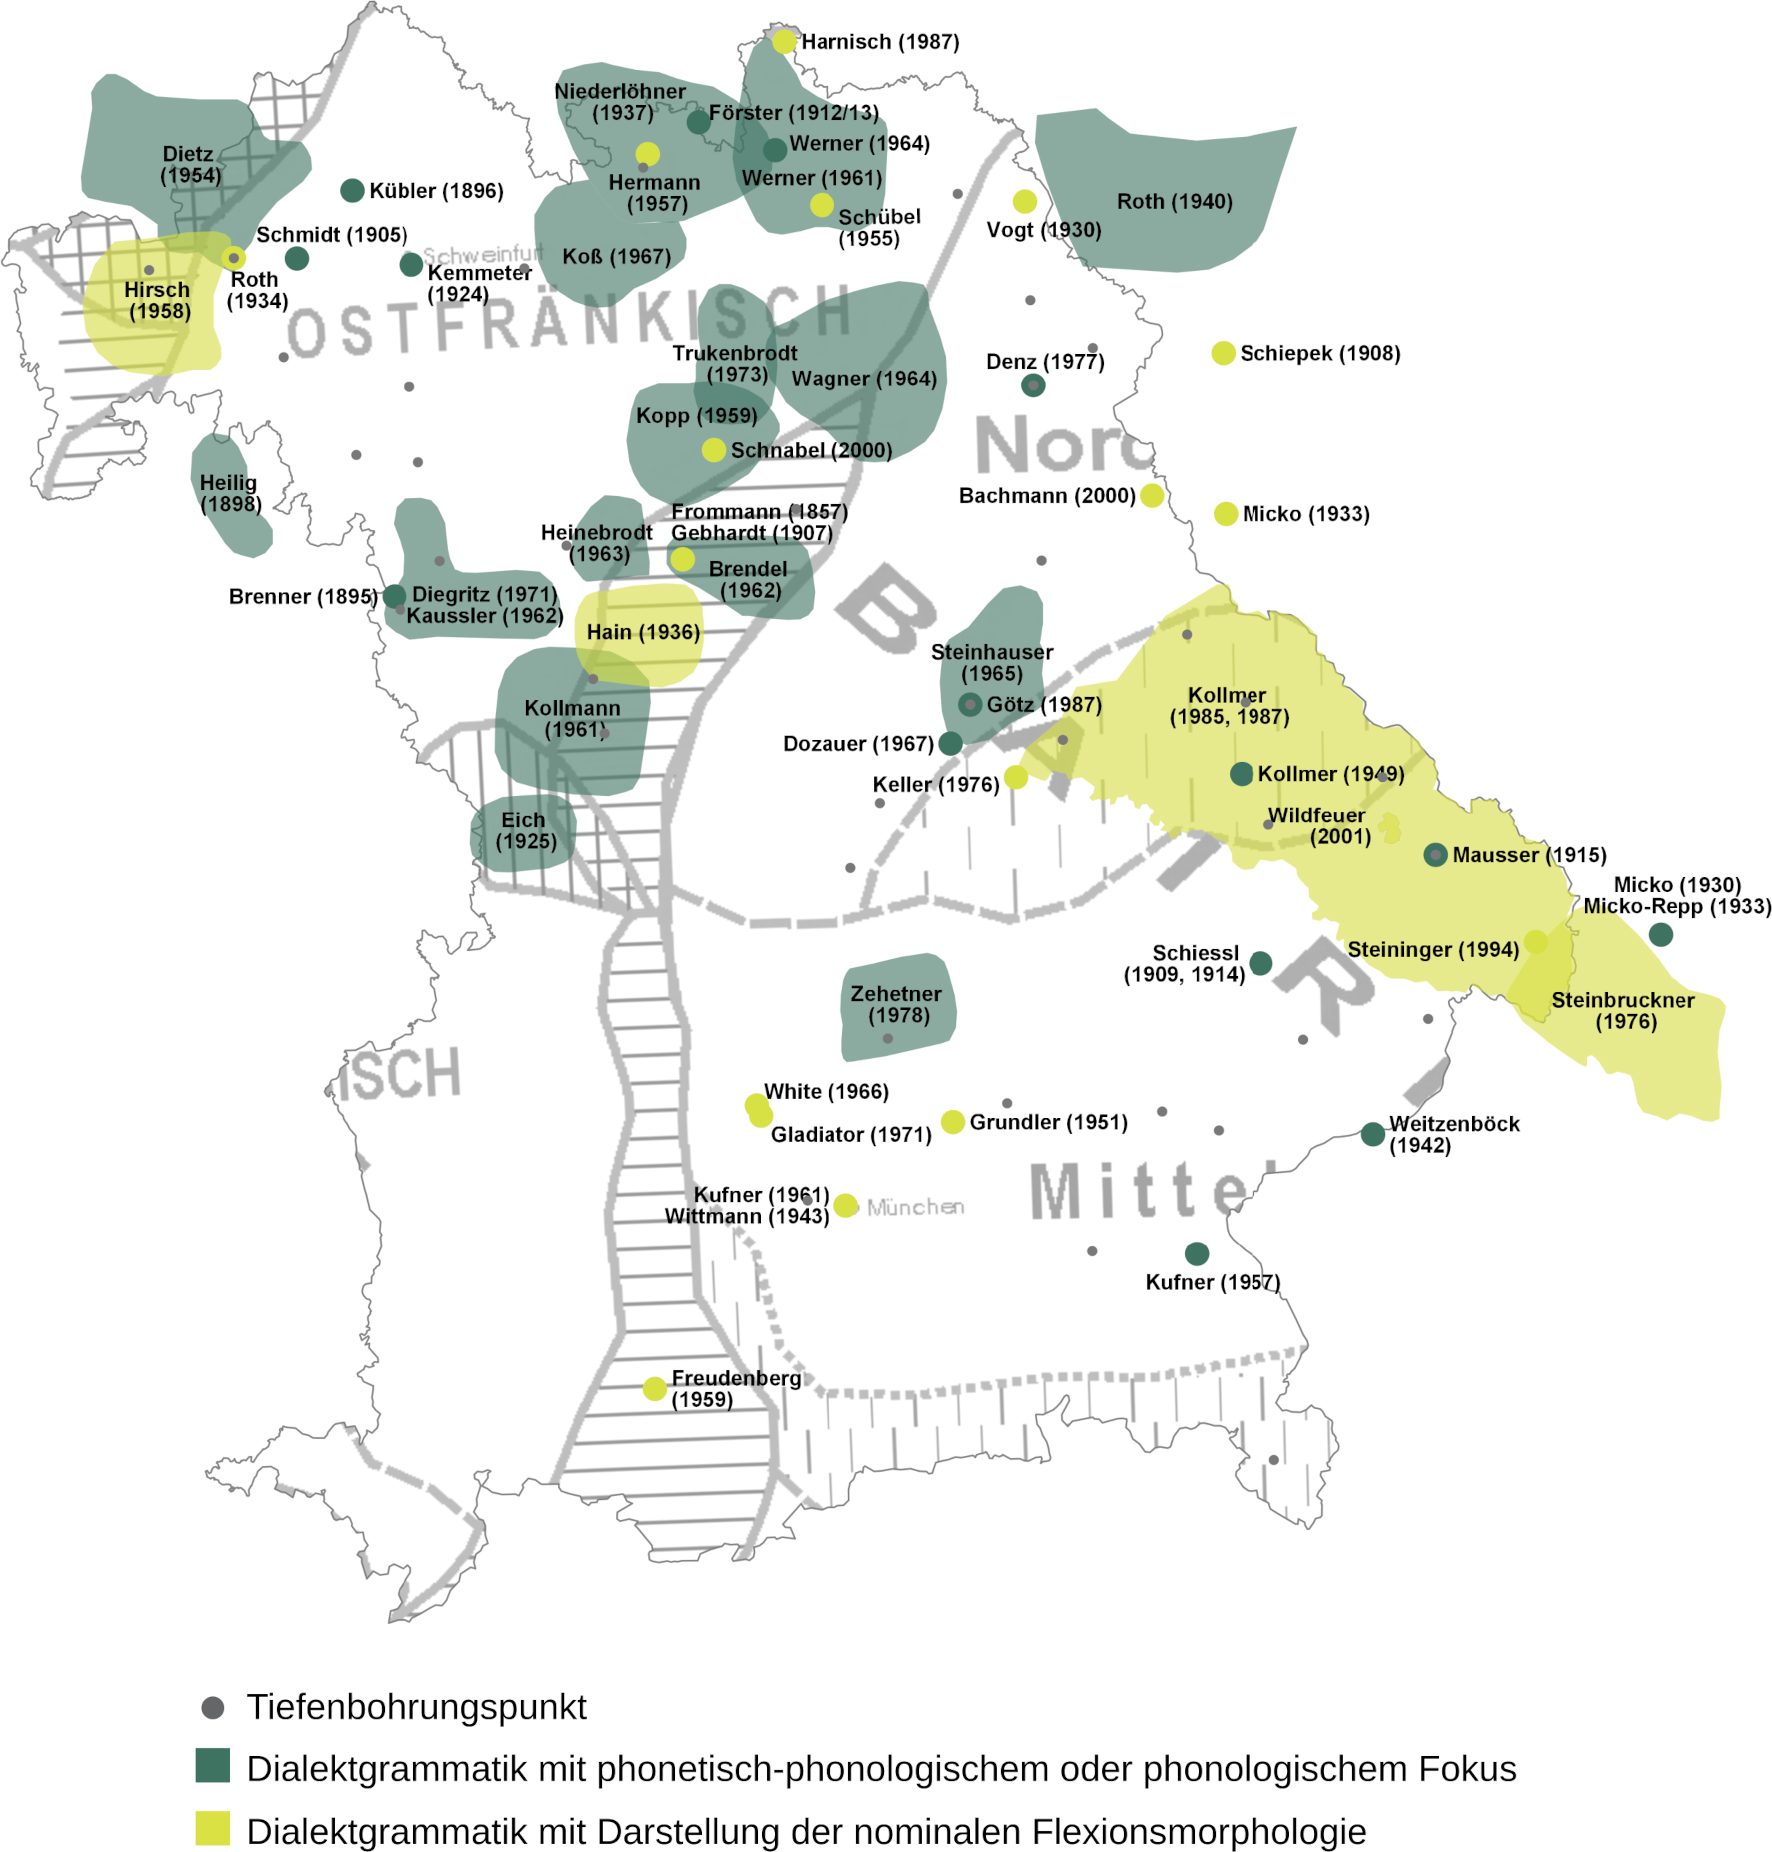
\includegraphics[width=\textwidth]{figures/Karte2.png}
\caption{Dialektgrammatiken zu den oobd. Dialekten Bayerns und \citegen{Wiesinger1983b} Dialekteinteilung}
\label{map:2}
\end{map}

Durch die \textit{Georeferenzierte Online-Bibliographie zur Areallinguistik} (\citealt{SchmidtEtAl2008ff}) ist es möglich, die relevanten dialektologisch-grammatischen Darstellungen im UG zu recherchieren.\footnote{Die \textit{Georeferenzierte Online-Bibliographie zur Areallinguistik} (GOBA) ist Teil des Projekts \textit{regionalsprache.de} und erreichbar über \url{www.regionalsprache.de}. Ich danke zudem den Kolleginnen und Kollegen des Deutschen Sprachatlas in Marburg und des REDE-Projekts für die Möglichkeit und Unterstützung bei der Recherche vor Ort.} Insgesamt wurde eine Auswahl von 65 Ortsmonografien, großräumigeren Landschaftsgrammatiken, Zeitschriftenaufsätzen sowie nicht-publizierten Hochschulschriften und Examensarbeiten ausgewertet (vgl. \mapref{map:2}). Berücksichtigt wurden dabei nicht nur Darstellungen der Flexionsmorphologie, sondern auch Lautlehren, die insbesondere im Oberofr. für ein relativ geschlossenes Gebiet vorhanden sind. Im Kontext einer flexionsmorphologischen Forschungsfrage haben diese zwar meist den Nachteil, dass Basisformen und flektierte Formen nur selten systematisch gegenübergestellt werden, allerdings ist die Darstellung phonologischer Prozesse (in den meisten Fällen ausschließlich oder mit Schwerpunkt im Bereich Vokalismus) mit Blick auf die morphophonologische Perspektive relevant.

\section{Datenaufbereitung und -auswertung}
\label{sec:6.3}
Hauptziel der Analyse ist es, durch den Vergleich von Realisierungsvarianten der Numerus- und Kasusmarkierung in den Ortsdialekten formale Gemeinsamkeiten und Unterschiede sowie -- auf einer übergeordneten Ebene -- Faktoren der Deklinationsklassenzusammensetzung herausarbeiten zu können. Dafür wurden die nicht-typisierten Rohdaten der BSA-Erhebungen als primäre Datenbasis für die 37 Ortspunkte in einer Datenbankanwendung gesammelt, aufbereitet und anschließend hinsichtlich diverser flexivischer und nicht-flexivischer Merkmale analysiert und annotiert (vgl. \sectref{sec:6.3.1}). Zusätzlich wurden im Rahmen der Datenauswertung die Wenker-Materialien und die relevanten Ortsgrammatiken als zusätzliche Evidenz herangezogen.

Die Materialquellen sind sowohl in der Transkription der Dialektbelege als auch in den angewandten Transkriptionsprinzipien ausgesprochen heterogen. Die Transkription der Originalbelege der unterschiedlichen Datenquellen wird sowohl in der Datenbankanwendung als auch in der folgenden Darstellung stets beibehalten und entsprechend interpretiert, um sie in der Analyse aufeinander beziehen zu können.\footnote{Aus Gründen der Lesbarkeit wird bei phonetischen Transkriptionen in der Regel auf die entsprechenden Klammern verzichtet. Mit diesem Ziel erscheinen bei transkribierten Phrasen und Syntagmen auch Leerstellen zwischen den Wortgrenzen.} Trotz einheitlichem Teuthonista-Notationssystem weist auch das BSA-Material von Teilprojekt zu Teilprojekt durchaus gewisse Eigenheiten in der Transkription auf, die ich in der Aufbereitung, insbesondere bei der Annotation der phonologischen und prosodischen Aspekte, zu berücksichtigen hatte (ausführlicher \sectref{sec:6.3.1.2}).

\subsection{Datenbank}
\label{sec:6.3.1}
Für die Dateneingabe und -auswertung wurde eine relationale Datenbank entworfen und mithilfe des Programms \textit{Microsoft Access 2010} aufgebaut. Diese Datenbank steht auf der Website der \textit{Bayerischen Dialektdatenbank} \textit{BayDat} zum Download zur Verfügung (\url{https://baydat.badw.de/materialien/nickel}). Das Format einer relationalen Datenbank wurde zur Datenanalyse und -ausgabe für die Untersuchung gewählt, weil es ein unkompliziertes und flexibles Hinzufügen oder Ändern einzelner Datensätze oder ganzer Annotationskategorien ermöglicht, was bei der Größe des zu untersuchenden Korpus und der Menge der Annotationskategorien von großem Wert und Effizienz war. In der Datenbankanwendung wurden die BSA-Belege aufbereitet und hinsichtlich vorab definierter flexionsmorphologischer, phonetisch-phonologischer, prosodischer, semantischer und außersprachlicher Kriterien analysiert und annotiert (vgl. \sectref{sec:6.3.1.4}). Die Datenauswertung erfolgt in Form von SQL-basierten Abfrageformularen, die das gezielte Sortieren und Durchsuchen der Datensätze zum Beispiel zu einzelnen Flexiven, Pluralmarkierungsverfahren oder einzelnen Konditionierungsfaktoren der Deklinationsklassenzusammensetzung ermöglichen.

\subsubsection{Aufbereitung der BSA-Daten}
\label{sec:6.3.1.1}
Die primäre Datenquelle der Untersuchung, die Rohdaten der Teilprojekte des \textit{Bayerischen Sprachatlas}, sind über die \textit{Bayerische Dialektdatenbank} \textit{BayDat} in einer zentralen Datenbankanwendung digital verfügbar. Zum Zeitpunkt der Datenaufbereitung war die neue und verbesserte Version der \textit{BayDat} noch nicht online; es wurde die nicht mehr aktive Version der Universität Würzburg genutzt.\footnote{Die neue \textit{BayDat}{}-Version ist über die Domain \url{https://baydat.badw.de/} erreichbar. Die nicht mehr aktive Version war über die Adresse \url{http://www.baydat.uni-wuerzburg.de:8080/cocoon/baydat/} verfügbar.} Ausgewertet wurden jene Fragen der Fragebücher der BSA-Teilprojekte, die Flexionsformen des Substantivs oder ganze Nominalphrasen behandeln. Die erhobenen Syntagmen sollten bei der Exploration dazu dienen, verschiedene Flexionsformen zu erheben, die ohne Kontext kaum abzufragen sind (vgl. \citealt[23]{Klepsch2013}). Wurden die Antworten der Gewährspersonen in Form ganzer Syntagmen transkribiert, wurden sie in dieser Form in das eigene Korpus aufgenommen. Mit 8.129 BSA-Datensätzen insgesamt enthält das Korpus Flexionsformen von 271 Lemmata, die entweder in allen der 37 Tiefenbohrungspunkten oder zumindest in einzelnen Teilprojekten abgefragt wurden (vgl. Anhang).

Die Rohdaten liegen in Form von Kodaten der Teuthonista-Transkriptionen der direkten Erhebungen des \textit{Bayerischen Sprachatlas} vor. Für eine elektronische Weiterverarbeitung wurden die handschriftlich transkribierten Belege in den einzelnen BSA-Projekten für jeden einzelnen Erhebungsort in eine \textsc{Ascii}{}-konforme Kodierung umgewandelt (\textit{American Standard Code For Information Interchange}), d.\,h. für die Kodierung der Teuthonista-Transkripte standen nur Zeichen aus dem \textsc{Ascii}{}-Zeichensatz zur Verfügung (näher hierzu \citealt[7--16]{Zimmermann2006}). Infolgedessen setzen sich die Teuthonista-Kodate im Wesentlichen aus Zeichen aus dem lateinischen Alphabet in Kombination mit Ziffern und Sonderzeichen zusammen, die die Diakritika der Teuthonista-Lautschrift abbilden (z.\,B. <a2.> für \teuthoo{a2.}{āͅ}). Als die BSA-Rohdaten in die Online-Plattform \textit{BayDat} eingebunden werden sollten, stellte sich die Schwierigkeit, dass für die Darstellung der Teuthonista-Transkripte in Windows-Systemen die Schriftart \textsc{TeuthoBd} aufgesetzt werden musste, die zwar ebenfalls auf dem \textsc{Ascii}{}-Zeichensatz basiert, aber eine andere Zuordnung der Zeichen verwendet als die Kodierung der Ortsdateien (vgl. \citealt[121]{Zimmermann2006}). Zwar war es möglich, die Kodate der ursprünglichen \textsc{Ascii}{}-Dateien automatisch in Zeichenfolgen für die Schriftart \textsc{TeuthoBd} umzuwandeln und gleichzeitig einige häufig auftretende Kodierfehler automatisch zu korrigieren, aber seltenere Kodierfehler konnten nicht behoben werden, weshalb sich zum Zeitpunkt der Datenaufbereitung dieser Untersuchung noch immer fehlerhafte Kodate in den \textit{BayDat}{}-Rohdaten finden ließen. 

Neben den potenziellen Kodierfehlern bestand zum Zeitpunkt der Datenaufbereitung eine weitere Schwierigkeit darin, dass die Ausgabe der Belege in \textit{BayDat} teilweise fehlerhaft ist.\footnote{Obwohl die Frage im entsprechenden Teilprojekt abgefragt wurde, erscheint die Meldung „Frage in diesem Projekt/Ort nicht erhoben“ oder es wird -- bei falscher Zuordnung von Fragenummer und Antwortbeleg -- ein anderer, nicht der Frage zugehöriger Beleg angezeigt. Die genannten Nachteile der alten \textit{BayDat}{}-Version werden im Zuge der Neu-Aufsetzung der \textit{BayDat} sukzessive behoben, was zukünftige Datenaufbereitungen erheblich erleichtern dürfte.} In beiden Fällen wurde das Vorhandensein der Belege in den Original-Fragebüchern der jeweiligen Untersuchungsorte überprüft und ggf. händisch kodiert. Auch nach manueller Überprüfung und Korrektur der Kodate ist mit einer gewissen Fehlerquote zu rechnen; diese Kodierfehler betreffen in erster Linie die Diakritika in der Teuthonista-Notation und damit phonetische Feinheiten, z.\,B. wie geschlossen ein /e/ realisiert wurde. Dies ist im Kontext einer morphologischen Untersuchung weniger schwerwiegend als in einer phonologischen, da hier v.\,a. relevant ist, dass dieses \textit{e} die Numerusinformation in Form eines Umlauts markiert. Sind Diakritika (z.\,B. bei der Notation von Vokalquantitäten) für das Pluralmarkierungsverfahren entscheidend, wurden im Zweifelsfall die Originaltranskripte zum Vergleich herangezogen.

\subsubsection{Typisierung der Teuthonista-Transkripte}
\label{sec:6.3.1.2}
Trotz des einheitlichen Teuthonista-Notationssystems gibt es in den einzelnen Teilprojekten des BSA Abweichungen im Transkriptionsverfahren und Spezifika einzelner Exploratoren (vgl. \citealt[22]{SNiB1}). Die große Stärke der Teuthonista-Notation, sämtliche phonetische Feinheiten abbilden zu können, wirft im Rahmen einer flexionsmorphologischen Untersuchung methodische und sprach\-sys\-tematische Fragen auf: Wann repräsentiert eine phonetisch differente Form zwischen Singular- und Pluralbeleg auch einen phonemischen Unterschied, der eine morphologische Unterscheidung kodiert? Wann handelt es sich um rein phonetische Variation ohne Funktionalität? Die Feinheit des Notationssystems mit beispielsweise vier Abstufungen der Vokalquantität und fünf Differenzierungen von Lenis- bzw. Fortisobstruenten stellt in der Praxis der Annotation von Pluralmarkierungsverfahren damit eine nicht geringe methodische Schwierigkeit dar, wie die Beispiele \REF{ex:6:1} und \REF{ex:6:2} illustrieren:

\ea\label{ex:6:1} \teuthoo{dA}{dα} \teuthoo{hu.2nd}{hūͅnd} – \teuthoo{dhu.nt5}{dhuͅnt̩} (‚Hund‘, Bernhardswald)
\ex\label{ex:6:2} \teuthoo{ha.2d}{hāͅd} – \teuthoo{he:<8d5}{hê{\doubleogonek}\klammerobenpost{}d̩} (‚Haut‘, Grafenkirchen)
\z

Es finden sich jeweils Kontraste in der Stammvokalquantität sowie Lenis"=Fortis"=Kontraste im Stammauslaut. Während die Kontraste in \REF{ex:6:1} zwischen Lang- und Kurzvokal respektive zwischen Lenis und leicht lenisierter Fortis bestehen, ergibt sich der Kontrast in \REF{ex:6:2} in der Notation eines Langvokals im Singular vs. einer eingeklammerten Halblänge im Plural, im Konsonantismus besteht der Kontrast zwischen Lenisplosiv vs. leicht fortisiertem Lenisplosiv. In der Annotation muss nun gewichtet werden, ob die z.\,T. minimale Variation, die transkribiert wurde, gleichermaßen als Beleg der Pluralmarkierungsverfahren Vokalquantitätskontrast und Lenis-Fortis-Kontrast klassifiziert werden kann oder ob es sich um eine rein phonetische Variation handelt, die aus Perspektive der Flexionsmorphologie vernachlässigt werden kann. Während der Bearbeitung der BSA-Bände bestanden ähnliche methodische Fragen, da die Transkripte auch für die Kartierung der Varianten typisiert werden mussten. Die folgenden Prinzipien der eigenen Typisierungs- und Klassifizierungspraxis orientieren sich daher an den Prinzipien des BSA (vgl. \citealt[6]{SMF2.1}, \citealt[18]{SUF1}):\largerpage

\begin{itemize}
\item Geklammerte Diakritika, z.\,B zur Markierung des Öffnungsgrades von Vokalen, werden wie ungeklammerte Diakritika behandelt, d.\,h. die Transkription \teuthoo{a)4}{a\klammeruntenpost{}̣} wird wie die Transkription \teuthoo{a4}{ạ} gewertet.\footnote{Reduzierungen von Grundzeichen und Diakritika in Form von Hochstellung des entsprechenden Zeichens (z.\,B. o\textsuperscript{α}) können (mit Ausnahme von <ʰ>) in der Schriftart \textsc{TeuthoBD} nicht dargestellt werden und konnten -- anders als in den BSA-Publikationen -- bei der Datenanalyse daher nicht berücksichtigt werden. Doppelt reduzierte Grundzeichen und Diakritika (z.B. \teuthoo{o}{o}\textsuperscript{(\teuthoo{a}{a})} wurden etwa im SMF als nicht vorhanden gewertet, diese Form der Notation kann in den \textsc{TeuthoBD}{}-Kodaten jedoch nicht mehr nachvollzogen werden.}
\item Halblängen (â) werden wie ganze Längen (ā) behandelt, d.\,h. im Beispielbeleg \REF{ex:6:2} würde kein Quantitätskontrast annotiert werden.
\item Vokalkürze wurde i.\,d.\,R. nicht gesondert notiert (Notation \teuthoo{a}{a}), in „besonderen (unerwarteten) Fällen“ (\citealt[163]{SBS1}) wurde Vokalkürze notiert (Diakritikum \teuthoo{a3}{ă}). Beide Notationen werden gleichermaßen als Kurzvokale behandelt.
\item Zwischenwertnotationen („Burger“) werden dem unteren Bestandteil zugeordnet, d.\,h. das Suffix \teuthoo{Å}{{\burgershwaalpha}} in der Pluralform \teuthoo{he94mÅd5\_Å}{he\klammeruntenpost{}̣m{\burgershwaalpha}d̩ʰ{\burgershwaalpha}} (‚Hemden‘, Mitteleschenbach) wird als α gewertet.
\item Abstufungen bei Lenes und Fortes werden als zweigliedriges Oppositionssystem behandelt: Lenes= \teuthoo{d;}{d͓͓} – \teuthoo{d,}{d͓} – \teuthoo{d}{d} – \teuthoo{d5}{d̩} – \teuthoo{d\%}{d͈}, Fortes= \teuthoo{t;}{t͓͓} – \teuthoo{t,}{t͓} – \teuthoo{t}{t} – \teuthoo{t5}{t̩} – \teuthoo{t\%}{t͈}. Die transkribierte Differenz in \REF{ex:6:2} würde damit nicht als Fortisierung annotiert, beide Plosive im Auslaut als Lenes behandelt werden (siehe hierzu auch \sectref{sec:7.1.2.3.1}).
\item Die Notationen \teuthoo{B}{{\btilde}} und \teuthoo{æ}{{\burgerbw}} werden (neben den Frikativen \teuthoo{w}{w}, \teuthoo{v}{v}) als Spirantisierungen von \teuthoo{b}{b} annotiert, z.\,B. \teuthoo{go<we}{ɡôwe} -- \teuthoo{gðo9.æe4n}{ɡ̩o\klammeruntenpost{}ͅ{\burgerbw}ẹn} (‚Gabel‘, Neukirchen am Inn)
\end{itemize}

\subsubsection{Mehrfachbelege und Variation im Datenmaterial}
\label{sec:6.3.1.3}
Im Normalfall wurde für jede Frage nur ein Antwortbeleg transkribiert. Wurden im Fragebuch mehrere Varianten transkribiert, so wurden diese entweder als eigene Datensätze in die Datenbank aufgenommen oder (v.\,a., wenn es sich um Aussprachevarianten handelte, die keine differente Form der Pluralmarkierung aufweisen) im Feld „Bemerkung“ des Formulars \textit{BSA-Belege} dokumentiert. Wenn für einen Untersuchungsort verschiedene Flexionsformen belegt waren, so erschien es von Anfang an sinnvoll, diese als eigene Datensätze in das Korpus aufzunehmen, da es sich um Belege intra-individueller oder (wenn mehrere Gewährspersonen beteiligt waren) inter-individueller Variation im Ortsdialekt handelte (siehe \citealt{Nickel2021}). Waren solche Varianten im Rohmaterial belegt, wurde stets im Originalfragebuch nachgeschlagen, ob es Exploratorenkommentare zu den varianten Formen gab, z.\,B. „spontan“, „Erinnerungsform“, „hochdeutsch“ o.\,ä. (vgl. \citealt[165f.]{SBS1}) Die Exploratorinnen und Exploratoren waren angehalten, insbesondere bei „lichtscheuen“ (Zitat aus den \textit{Grundsätzen für Sprachatlasaufnahmen} von Robert Hinderling, zitiert nach \citealt[48]{Schmuck2014}), d.\,h. schwer zu elizitierenden Lauten und Formen auf Selbstkorrekturen der Gewährspersonen zu achten und diese als solche kenntlich zu machen. Hat sich die Gewährsperson korrigiert, so wurde der korrigierte Beleg als Datensatz aufgenommen, der (Spontan-)Beleg wurde in das Feld „Bemerkungen“ aufgenommen und als solcher gekennzeichnet. Außerdem wurden die Kommentare der Exploratoren in das Feld „Bemerkungen“ aufgenommen, da sie Hinweise für eine Verortung der varianten Formen in der horizontalen oder vertikalen Dimension sind.

\subsubsection{Datenannotation und -auswertung}
\label{sec:6.3.1.4}
Den Untersuchungsgegenstand stellen das Substantiv und die syntaktische Einheit Nomi\-nal\-phrase bestehend aus Definitartikel und Substantiv dar. In die Datenbankanwendung wurden die BSA-Transkripte (Nom.Sg. und Nom.Pl. des Substantivs, ggf. Formen der obliquen Kasus und Diminutivformen) als isolierte Belege oder ganze Nominalphrasen eingepflegt, lemmatisiert und mit der Information zum Erhebungsort verknüpft. Die Analyse der Daten erfolgte durch die Annotation verschiedener flexionsmorphologischer und nicht-flexivischer Merkmale. Zur Analyse der Flexion gehören die konkreten Pluralmarker, aufgeschlüsselt nach möglichen Kontrasten im Vokalismus (Qualität und Quantität), im Konsonantismus sowie möglichen Suffixen, dem abstrahierten Typ des Pluralkodierungsverfahren (Null, additiv, modulativ oder die diversen kombinierten Verfahren) sowie der dialektalen Deklinationsklasse. Neben der Analyse der Pluralallomorphie besteht das zweite Untersuchungsziel darin, die Konditionierungsfaktoren der Deklinationsklassenzusammensetzung im Flexionssystem der Tiefenbohrungspunkte herauszuarbeiten. Der Analyseaspekt knüpft an die Forschung zur Konditionierung von Deklinationsklassen und Deklinationsklassenwandel im Schriftdeutschen und in den Dialekten an. Die Kategorien der Datenannotation bilden die Ergebnisse des aktuellen Forschungsstandes ab, indem folgende mögliche Konditionierungsfaktoren ausgewertet werden: Genus,\footnote{Liegt der Dialektbeleg in Form einer Nominalphrase mit Artikel vor, wurde die Form des Artikels hinzugezogen, um die Genuszugehörigkeit des Lexems im Ortsdialekt analysieren zu können. Wurde das Genus des Lexems durch einen metasprachlichen Kommentar angegeben, ist dies ebenfalls berücksichtigt. Stehen weder morphosyntaktischer Kontext noch metasprachliche Angaben zur Verfügung, musste das Genus ausgehend vom Standard oder unter Berücksichtigung von Dialektgrammatiken oder vorhandenen Sprachatlanten annotiert werden. Die dialektale Genuszugehörigkeit gilt dann nicht als gesichert und wird durch Einklammerung der Genuszuweisung („(fem.)“, „(mask.)“, „(neutr.)“) markiert.} prosodisch"=phonologische Aspekte (u.\,a. Silbenanzahl und -auslaut), morphologische Aspekte (Wortbildung, Singularstammform) sowie semantische Merkmale. Durch den Aufbau der Datenbank und die differenzierte Form der Annotation  ist es möglich, die Dialektbelege nach einzelnen Merkmalen (z.\,B. Pluralmarkierung bei Kontraktion des Singularstammes) oder einer Kombination von Merkmalen (z.\,B. Pluralmarkierung von \textit{n}{}-erweiterten Substantiven mit kontrahiertem Singularstamm) in den Auswertungsformularen zu sortieren und anzuzeigen. Die Abfrageformulare ermöglichen es, -- je nach Einstellung des Filters -- die absolute Anzahl der relevanten Belege abzulesen. Weitere statistische Auswertungen erfolgten dann außerhalb der Datenbankanwendung.

\subsection{Kartierung}
\label{sec:6.3.2}
Die Auswertungen werden durch Sprachkarten ergänzt, um die areale Dimension der Variation, und möglicherweise die Dialektspezifik einzelner Phänomene zu visualisieren. Diese Sprachkarten sind ein Instrument der Datenauswertung, sie sind daher weniger Untersuchungsziel an sich als ein Zwischenergebnis. Zur Kartierung wurden Beleglisten aus der \textit{Access}-Datenbankanwendung in das Tabellenkalkulationsprogramm \textit{Excel} exportiert und für die Kartierung aufbereitet. Die Erstellung der Karten erfolgte mit dem \textit{REDE SprachGIS} (\citealt{SchmidtEtAl2008ff}), das den Import von Datensätzen im CSV-Format und damit auch das automatische Kartieren der eigenen Beleglisten ermöglicht.\footnote{Die Farbgebung der Karten basiert stets auf den durch die Anwendung \textit{iWantHue: Colors for data scientists} (\url{https://medialab.github.io/iwanthue/}) empfohlenen Farbspektren für distinkte Farben.}
